\section{Foundations}

Mr Shannon's information theory is based on a number of mathematical principles. Some choices have been made, and we'll explain them below. The founding principles can be summed up roughly as the choice of the logarithm and the use of entropy. To make these principles easier to understand, we have developed solutions in Python, notably by implementing a bot that plays the game Wordle.

\subsection{The logarithmic function}

In his paper \cite{shannon1948mathematical}, Claude Shannon addresses the fundamental problem of communication, which technically consists of reproducing a message selected at one point from another point. He stresses that the semantic aspects of communication, such as the meaning of messages, are unimportant. What matters is that the actual message comes from a set of possible messages, and the system must be designed to work for every possible selection.

To quantify the information produced when a message is selected from a set, Shannon proposed a measure based on the logarithm. This measure is practical for several reasons. Firstly, it is more practically useful, as it allows important engineering parameters such as time, bandwidth and number of relays to be expressed linearly. Secondly, it better matches our intuition as to the appropriate measurement, as it allows linear comparisons with common standards. Finally, it is mathematically more suitable, as many limit operations are simple in logarithmic terms but would require awkward reformulation in terms of the number of possibilities.

The choice of logarithmic base corresponds to the choice of a unit for measuring information. The use of base 2 leads to units called "bits", while base 10 leads to units called "decimal digits". In certain analytical contexts, base "e" may also be used, giving rise to units called "natural units". Switching from one base to another simply requires multiplication by the logarithm of the ratio between the bases.In the context of Wordle, the words are a sequence of letters that can be converted to bits so we will use the base 2.

An alternative to the logarithm would be the square root. In some cases, this function could be used to give less weight to extreme values.



\begin{figure}[!ht]
\centering
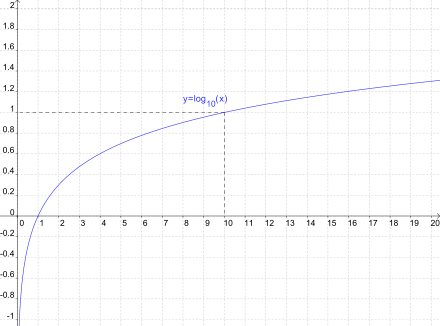
\includegraphics[scale=0.7]{images/logarithme.png}
\caption{logarithm curve \cite{wiki_log}}
\label{logarithm}
\end{figure}

\newpage

\subsection{Entropy and a ``word game`` implementation}

To explain exactly what entropy is, what better way than to create a bot that has to make choices. Because that's exactly what entropy is, a measure of uncertainty.

Word game or Wordle is a game in which you have to find a random word, and each time you make a move, you receive feedback that lets you know whether for each letter 0: it's in the right place, 1: it's not in the right place, 2: it's not present or no longer present in the word. The words we play are defined in a text document (5-letter English words).
We implemented this game in python and created a bot capable of making choices thanks to entropy.
In our case, each letter of the word is a symbol.
In the context where each symbol is independent, the entropy formula is as follows.

$$-\sum p_i \log(p_i)$$

where pi is the probability of symbol i.

For a word, we'll calculate symbol by symbol, the probability that it will appear (i.e. its frequency at that location) and then apply the formula. Finally, we add up each result, giving the word's entropy.
 
Entropy varies between 0 and 1, when using base 2. When it comes to comparing them and making a choice, the one that tends most towards 0 is the most likely. 
For our context: in the list of available words, we calculate and compare the entropy of each word. Then we use the word with the highest entropy to play and get the next feedback (using the maximum entropy allow us to test the widest sample). 

This process makes it possible to make the best possible choice when feedback is already available. But what about the first choice? We have several options for several results. 

\begin{enumerate}
    \item Calculate the entropy of each word in the complete list, then select the word with the highest entropy.
    \item Put each letter where its frequency is highest.
    \item Calculate the "pairs" of symbols most repeated at each location.
\end{enumerate}

\begin{figure}[!h]
\centering
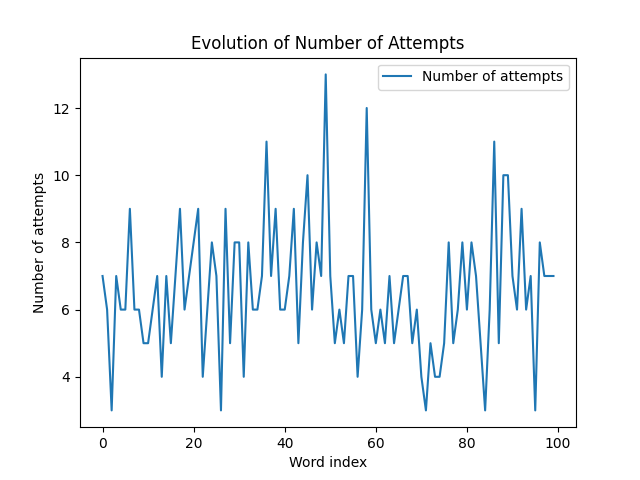
\includegraphics[scale=0.7]{images/start1.png}
\caption{100 first words, for start word 1 (50\% win rate)}
\label{start1}
\end{figure}

\begin{figure}[!h]
\centering
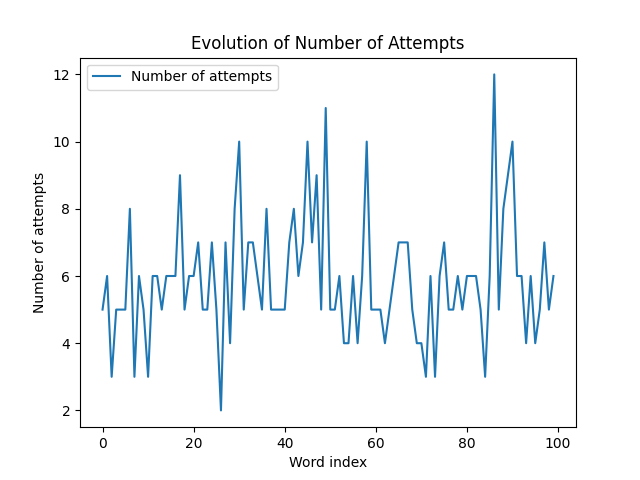
\includegraphics[scale=0.7]{images/start2.png}
\caption{100 first words, for start word 2 (70\% win rate)}
\label{start2}
\end{figure}

\newpage

It's obvious that the second "first word technique" is the best, giving approximately 70\% of win, against 50\% for the first. (we didn't implement the third)

\begin{figure}[!h]
\centering
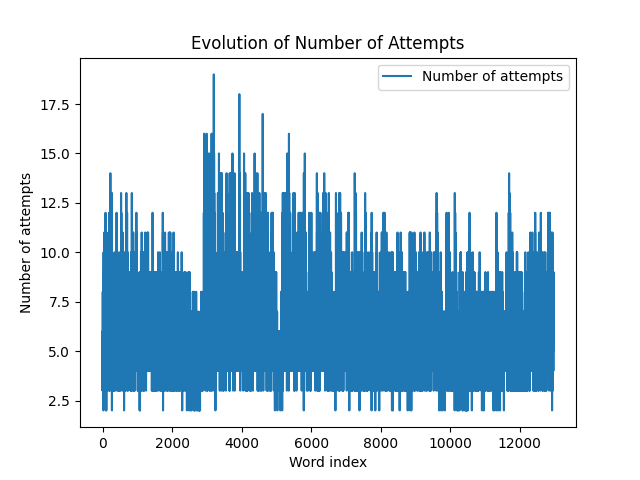
\includegraphics[scale=0.7]{images/start2-total.png}
\caption{all words in list, for start word 2}
\label{total}
\end{figure}

Note that these comparisons and calculations are based on the given list of 5-letter words. An interesting approach would have been to have the same statistics but on the whole English language. In this way, the frequencies of symbols and "blocks" of symbols would not be the same.

Once it has the best first word, the bot will sort the list of possible words according to feedback, then play the word with the highest entropy from this list. 
\subsection{Shannon's theorem}\cite{shannon1948mathematical}

So what is Shannon's objective? 
Through logarithmic entropy, Claude Shannon showed us that a certain amount of redundancy was necessary to be sure of getting the right message from the available list. However, thanks to data compression, we can greatly reduce redundancy without any loss of efficiency or accuracy.
But the aim behind all this is to maximize the variable C, which represents the maximum transmission capacity for a given time.

\subsection{Capacity}

The capacity C is defined in the Theorem 1 by $C = logW$, $W$ being the Determinant of the matrix of a communication system defined by:

Theorem 1: Let $b_{ij}^{(s)}$ be the duration of the $s^{th}$ symbol which is allowable in state i and leads to state j.
Then the channel capacity C is equal to $logW$ where $W$ is the largest real root of the determinant equation equation: $|\sum_s W{-b_{ij}^{(s)}} \delta{_{ij}}| = 0$

Where $\delta{_{ij}} = 1$ if $i = j$ 0 otherwise.